\def\ptitle{ArmoniK : An Open-Source Solution for Computation Orchestration and Distribution} % Title
\def\pauthor{Jérôme Gurhem} % Author
\def\pcollaborators{Wilfried Kirschenmann} % Advisors
\def\pteam{} % Team
\def\pinstitute{Aneo, Boulogne-Billancourt, France} % Affiliation
\def\pdate{Jeudi 26 Juin, 2025} % Date

\pdfobjcompresslevel=0
\documentclass[final]{beamer}
\usepackage[orientation=portrait,size=a0,scale=1.4]{beamerposter}
\usepackage[utf8]{inputenc}
\usepackage[sfdefault]{roboto}
\usepackage[english]{babel}
\usepackage{amsmath, amsthm, amssymb, array, booktabs, grffile, latexsym, tabularx, xspace, hyperref}
\newcolumntype{Z}{>{\centering\arraybackslash}X}
\newcommand{\pphantom}{\textcolor{ta3aluminium}}
\newlength{\columnheight}

\def\purl{\url{https://2025.compas-conference.fr/}}
\def\pdate{\Large Compas, 26 juin 2025} % Date
\def\pmail{\Large Bordeaux ~~~~~~}

\mode<presentation>{\usetheme{COMPAS}}
\title[\ptitle]{\texorpdfstring{\huge \ptitle}{\ptitle}}
\author[\pauthor]{\pauthor\ -\ \padvisors}
\institute[\pinstitute]{\pteam\ -\ \pinstitute}
\date[\pdate]{\pdate}
\setlogo{\plogo}
\setauthorurl{\purl}
\setauthoremail{\pmail}


\usepackage{listings}
\usepackage{tikz}
\usepackage{svg}
\usepackage{relsize}
\usetikzlibrary{positioning, fit, backgrounds, shapes, arrows.meta}

\graphicspath{{./fig/}} % Figures and logos directory
\setlength{\columnheight}{700ex} % Tweak this value if columns are too long/short (should be okay with 588ex)

\definecolor{pykeyword}{rgb}{0.25, 0.3, 0.85}
\definecolor{pycomment}{rgb}{0.0, 0.6, 0.0}
\definecolor{pystring}{rgb}{0.65, 0.1, 0.1}
\definecolor{codebg}{rgb}{0.97, 0.97, 0.97}
\lstdefinestyle{pythonstyle}{
  language=Python,
  basicstyle=\ttfamily\scriptsize,
  keywordstyle=\color{pykeyword}\bfseries,
  commentstyle=\color{pycomment}\itshape,
  stringstyle=\color{pystring},
  backgroundcolor=\color{codebg},
  showstringspaces=false,
  breaklines=true,
  frame=single,
  rulecolor=\color{gray},
  tabsize=2,
  morekeywords={self}, % highlight custom keywords
}

\lstset{style=pythonstyle}



\begin{document}
\begin{frame}[fragile]

  \begin{columns}[T]
    \begin{column}{.49\textwidth}
      \begin{beamercolorbox}[center,wd=\textwidth]{postercolumn}
        \begin{minipage}[T]{.96\textwidth}
            \begin{block}{Objectives}
              \begin{itemize}
                \item Provide an Open-Source, scalable platform for executing distributed workloads efficiently on heterogeneous infrastructures
                \item Simplify the development and deployment of distributed computing codes
                \item Maximize resource utilization across private/public clouds and HPC clusters
                \item Provide a high-level abstraction for developers
              \end{itemize}
            \end{block}
          \end{minipage}
      \end{beamercolorbox}
      \vfill
    \end{column}
    \begin{column}{.49\textwidth}
      \begin{beamercolorbox}[center,wd=\textwidth]{postercolumn}
        \begin{minipage}[T]{.96\textwidth}
          \begin{block}{Key Benefits and Outcomes}
            \begin{itemize}
                \item Smart orchestration ensures efficient task execution at scale
                \item Modular, elastic architecture adapts to workload variation
                \item Built-in observability enables reliability and performance monitoring
                \item Empowers the next generation of high-performance, data-intensive applications
            \end{itemize}
          \end{block}
        \end{minipage}
      \end{beamercolorbox}
    \end{column}
  \end{columns}
  \vfil

  \begin{center}
  \begin{minipage}[T]{.975\textwidth}
  \begin{block}{ArmoniK Positionning in HPC}
    \centering
    \includegraphics[width=.8\textwidth]{armonik_framework.pdf}
  \end{block}
  \end{minipage}
  \end{center}
  \vfill

  \begin{columns}[T]
    \begin{column}{.49\textwidth}
      \begin{beamercolorbox}[center,wd=\textwidth]{postercolumn}
        \begin{minipage}[T]{.96\textwidth}
          \begin{block}{Dynamic Graph}
          \begin{itemize}
              \item Dependency graph is not fully known when scheduling starts
              \item Submissions can happen anytime
              \item Tasks can submit new tasks
              \item Tasks can delegate the production of their output to their new tasks
          \end{itemize}
          \centering
          \includesvg[width=0.7\textwidth, pretex=\relscale{0.65}]{subtasking.svg}
          \end{block}

            % \begin{block}{Task Definition in ArmoniK}
            % \lstinputlisting[language=Python]{task-based-programming.py}
            % \end{block}

            % \begin{block}{Dynamic Graph Example}
            % \lstinputlisting[language=Python]{subtasking.py}
            % \end{block}
        \end{minipage}
      \end{beamercolorbox}
    \end{column}
    \begin{column}{.49\textwidth}
      \begin{beamercolorbox}[center,wd=\textwidth]{postercolumn}
        \begin{minipage}[T]{.96\textwidth}
            \begin{block}{Other features}
                \begin{itemize}
                \item \textbf{Observability}: GUIs, CLIs, monitoring APIs, metrics, logs, and traces to understand of the state of the system
                \item \textbf{Portability}: Easy to transfer an application from one environment to another
                \begin{itemize}
                    \item Officially supported languages: C\#, C++, Python, Rust, Java, and JavaScript
                    \item Tasks on different architectures (x86, ARM, GPU, Linux, Windows), applications, environments
                \end{itemize}
                \item \textbf{Malleability}: Support dynamic reconfiguration of the number of allocated resources during execution without interruption
                \item \textbf{Resource Sharing}: Allow sharing resources between applications to execute as many as possible at the same
                \item \textbf{Modularity}: Modules can be swapped without modifying ArmoniK's code to suit user neeeds and constraints
                \end{itemize}
            \end{block}
        \end{minipage}
      \end{beamercolorbox}
    \end{column}
  \end{columns}
  \vfill


  \begin{columns}[T]
    \begin{column}{.49\textwidth}
      \begin{beamercolorbox}[center,wd=\textwidth]{postercolumn}
        \begin{minipage}[T]{.96\textwidth}
          \begin{block}{Computations/Comm Overlapping}
              \begin{itemize}
              \item ArmoniK is responsible for tasks input and output data management
              \item Allow for automatic communication + scheduling/task execution overlapping
              \item Automatic Uncoordinated Checkpointing
              \end{itemize}
              \vspace{3ex}
              \centering
              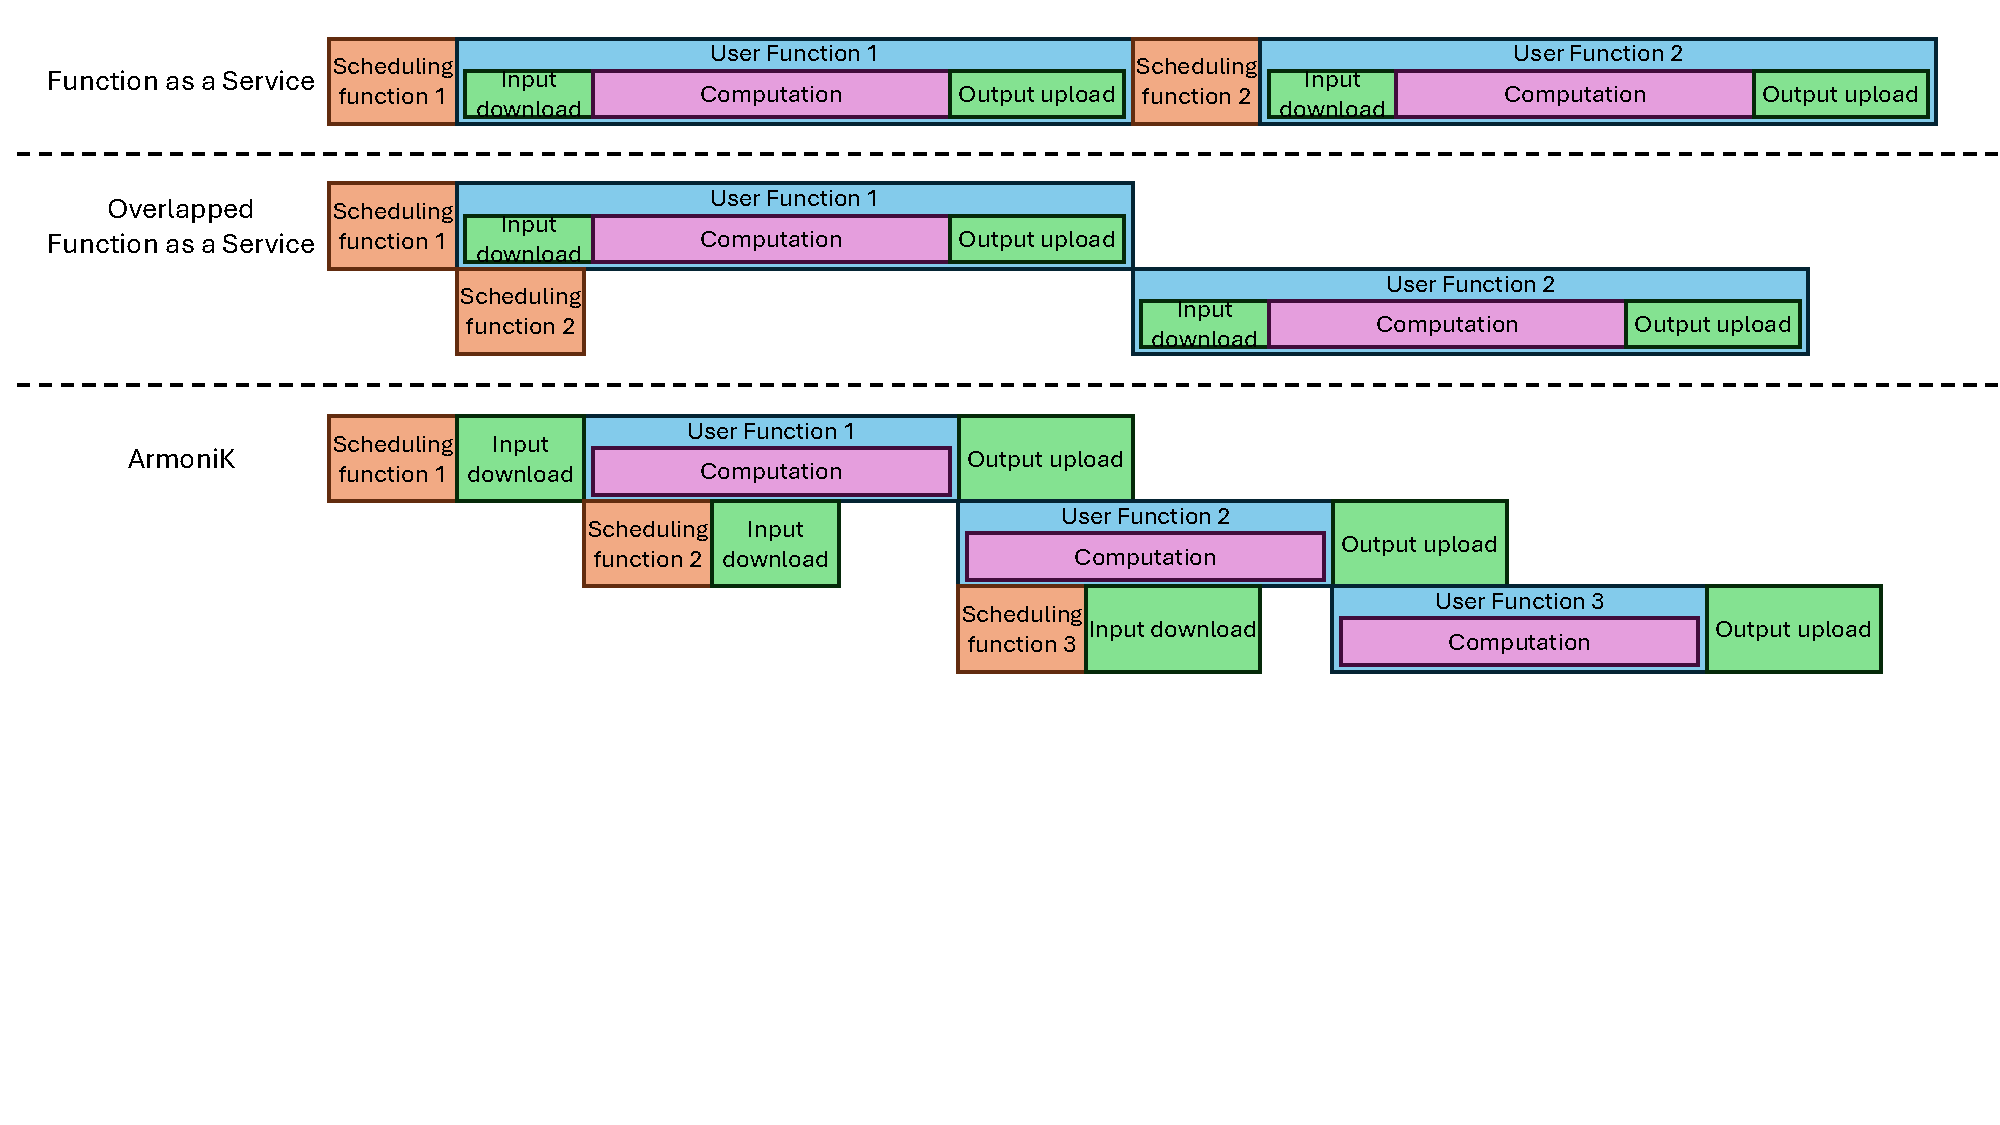
\includegraphics[width=\textwidth, trim={0 6.5cm 0 0}, clip]{pipelining AK 2.pdf}
          \end{block}
        \end{minipage}
      \end{beamercolorbox}
    \end{column}

    \begin{column}{.49\textwidth}
      \begin{beamercolorbox}[center,wd=\textwidth]{postercolumn}
        \begin{minipage}[T]{.96\textwidth}
            \begin{block}{Fault Tolerance}
              \begin{itemize}
              \item Works without interruption even when one or more nodes fail
              \item Allow support for preemptible computing resources
              \item Automatic and efficient task retry on failure
              \item Each curve represents a percentage of preempted instances
              \end{itemize}
              \begin{figure}
                \centering
                \includesvg[width=0.75\textwidth]{bench_preemption.svg}
              \end{figure}
            \end{block}
        \end{minipage}
      \end{beamercolorbox}
    \end{column}
  \end{columns}



  \begin{center}
  \begin{minipage}[T]{.975\textwidth}
  \begin{block}{Performance \& Scalability}
    \begin{columns}[T]
      \begin{column}{.49\textwidth}
      \begin{itemize}
        \item Indep : independent tasks workload
        \item Graph : nested fork-join workload
      \end{itemize}
      \begin{figure}
      \centering
      \includesvg[width=0.8\textwidth]{bench_scalability.svg}
      \end{figure}
      \end{column}

      \begin{column}{.49\textwidth}
      \begin{itemize}
        \item Cumulative distribution functions (CDFs) of round-trip latency
        \item Batched submissions of 1, 10, and 100 independent zero-work tasks
      \end{itemize}
      \begin{figure}
      \centering
      \includesvg[width=0.8\textwidth]{bench_roundtrip_latency.svg}
      \end{figure}
      \end{column}
    \end{columns}

  \end{block}
  \end{minipage}
  \end{center}
  \vfill

  \vskip1ex
\end{frame}
\end{document}